\section{方法与实验设计}
\subsection{低秩参数适应：把数学落实为可验证的实现}
模型参数是计算输出时使用的数字。前向计算得到输出，反向传播计算损失对参数的梯度，优化器才真正修改参数。LoRA 是参数高效微调的一种方式：冻结原来的大权重，只训练附加的小矩阵。\cite{lora,lorasurvey}

对列向量输入 $\boldsymbol{x}\in\mathbb{R}^{d_{\mathrm{in}}}$，原线性层为 $W\boldsymbol{x}+\boldsymbol{b}$。LoRA 引入
\[
W\in\mathbb R^{d_{\mathrm{out}}\times d_{\mathrm{in}}},\qquad
A\in\mathbb R^{r\times d_{\mathrm{in}}},\qquad
B\in\mathbb R^{d_{\mathrm{out}}\times r}.
\]
\begin{align}
\Delta W&=\frac{\alpha}{r}BA,\quad r>0,\label{eq:lora-zh}\\
\boldsymbol{y}&=W\boldsymbol{x}+\boldsymbol{b}
+\frac{\alpha}{r}BA\boldsymbol{x}.\label{eq:lora-forward-zh}
\end{align}
$r$ 是中间空间的宽度，也是修正矩阵秩的上界；$\alpha/r$ 控制新增路径的幅度。$A$ 先把输入映射到较小空间，$B$ 再映射回输出维度。训练时更新 $A,B$，原来的 $W,\boldsymbol b$ 保持冻结。

\begin{minipage}{\linewidth}
\par\noindent\begin{minipage}{\linewidth}
\begin{center}
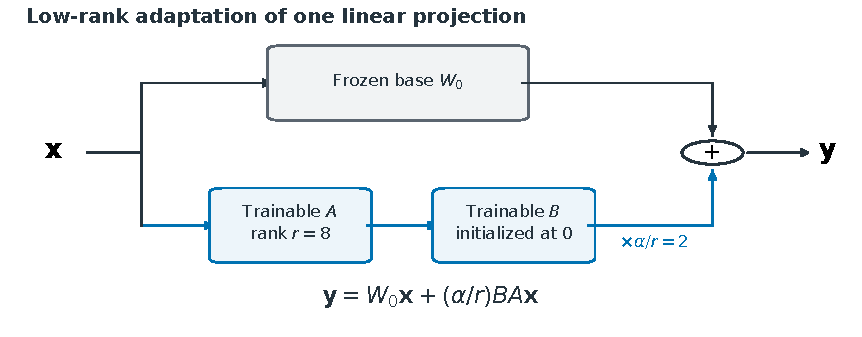
\includegraphics[width=146mm]{../../figures/lora_mechanism.pdf}
\end{center}
\figcaption{fig:lora-zh}{LoRA 原路径与低秩修正路径。两条路径的输出相加；示意图用于解释式~\eqref{eq:lora-forward-zh}，不表示已经完成训练。}
\end{minipage}\par

\end{minipage}

忽略偏置，原权重包含 $d_{\mathrm{in}}d_{\mathrm{out}}$ 个参数，LoRA 新增 $r(d_{\mathrm{in}}+d_{\mathrm{out}})$ 个。若两个维度均为 1024、$r=8$，原权重为 1,048,576 个参数，新增为 16,384 个。但完整模型仍要保存冻结权重并参与计算，所以可训练参数比例不等于显存节省比例。

实现采用随机初始化 $A$、零初始化 $B$，使初始 $BA=0$，保持原层输出。推理时可合并 $W\leftarrow W+\Delta W$；之后必须关闭新增路径，避免重复相加。PyTorch 的批量输入按行存放，关闭 dropout 时对应
\[
Y=XW^{\mathsf T}+\boldsymbol{1}_m\boldsymbol b^{\mathsf T}
 +\frac{\alpha}{r}XA^{\mathsf T}B^{\mathsf T}.
\]
六处具体实现、$r=0$ 的边界处理和手工实现输出保存在附录~\ref{app:implementation-zh}。

\subsection{学习率与批大小：设计依据，而非已完成的消融实验}
学习率决定每次参数更新的尺度。最简单的梯度下降写成
\begin{equation}
\boldsymbol{\theta}_{t+1}
=\boldsymbol{\theta}_t-\eta\nabla_{\boldsymbol{\theta}}\mathcal L(\boldsymbol{\theta}_t).
\label{eq:learning-rate-zh}
\end{equation}
这里 $\eta$ 是学习率，梯度给出损失对参数变化的敏感方向；实际 Adam 还利用历史梯度。学习率较小可能更温和，但在有限步数内进展较慢；较大可能加快初期变化，也可能越过合适区域或使优化不稳定。

批大小表示一次有效更新使用多少样本。若固定 1,024 条数据且不做梯度累积，批大小 8 对应 128 次更新，批大小 64 只有 16 次更新。因此比较批大小时，必须说明固定的是数据量、更新次数还是计算预算。较大批量通常降低梯度波动，却可能增加显存需求；较小批量节约单次显存，但梯度更有噪声，设备利用率也可能较低。文本长度同样会影响成本。

\textit{LoRA Without Regret} 在其研究设置中观察到：LoRA 合适的学习率约为全参数微调的十倍；一些大批量设置会扩大差距，单纯提高秩也未消除差距。\cite{lorablog} 这些是该文的经验结果，不是所有任务通用的规则。本研究据此理解学习率、秩、缩放和批量的相互影响，但只采用一个训练配置，没有实测学习率或批大小的优劣。

\subsection{PPO 与外部奖励}
LoRA 决定哪些参数可以更新；PPO 决定怎样根据奖励更新它们。实际训练使用 OpenRLHF 集成的 PEFT 适配器，手写 LoRA 层用于理解和功能验证；二者不是把同一个手写层直接替换进整个 PPO 框架。这里使用可执行的算术评分规则，没有收集人类偏好数据。

\par\noindent\begin{minipage}{\linewidth}
\tablecaption{tab:roles-zh}{训练中的四种角色及其区别。}
\begin{tabularx}{\linewidth}{@{}P{32mm}Y@{}}
\toprule
\tablehead \key{角色} & \key{作用}\\
\midrule
Actor：策略模型 & Qwen 加 LoRA，逐个 token 生成回答；token 是模型处理文字的基本单位。\\
Critic：价值模型 & 预测后续回报，帮助计算行为相对预期的优势。\\
Reference：固定参照 & 保留初始模型，用于约束策略偏离。\\
Reward：外部评分 & 本地 HTTP 服务核对首行整数，给出 0 或 1 的任务奖励。\\
\bottomrule
\end{tabularx}
\end{minipage}\par


PPO 比较当前策略和生成这一批样本时的旧策略，裁剪目标为\cite{ppo}
\begin{align}
\rho_t(\boldsymbol{\theta})
&=\frac{\pi_{\boldsymbol{\theta}}(a_t\mid s_t)}
{\pi_{\mathrm{old}}(a_t\mid s_t)},\\
J_{\mathrm{clip}}(\boldsymbol{\theta})
&=\mathbb E_t\!\left[
\min\!\left(\rho_t\widehat A_t,\,
\operatorname{clip}(\rho_t,1-\epsilon,1+\epsilon)\widehat A_t\right)\right].
\label{eq:ppo-zh}
\end{align}
$s_t$ 是当前上下文，$a_t$ 是生成的 token，$\widehat A_t$ 是优势估计。概率比值 $\rho_t$ 与 LoRA 的秩 $r$ 不是同一个量。例如概率从 0.2 增至 0.3，概率比值为 1.5；当 $\epsilon=0.2$，裁剪后的比值为 1.2。裁剪限制目标收益，却不严格保证策略距离一定小于某个值。

本实验使用 Critic 和 GAE。忽略终止位置的掩码时，可按下面两步理解优势：
\[
\delta_t=\widetilde r_t+\gamma V(s_{t+1})-V(s_t),\qquad
\widehat A_t=\sum_{\ell=0}^{T-t-1}(\gamma\lambda)^\ell\delta_{t+\ell}.
\]
其中 $\widetilde r_t$ 是包含相对 Reference 约束的实际奖励；优势衡量的是“获得的反馈比原先预计好多少”。PPO 的旧策略只对应当前采样批次，Reference 则固定为初始模型，二者不能混用。初始 KL 系数为 $\beta=0.01$。

\subsection{算术任务与配对验证协议}
\path{policy_adaptation/prepare_ppo_data.py} 以种子 1234，从 $0\le a\le b<50$ 的加法数对中产生 512 道训练题和 128 道开发验证题。两组互不交叠，交换加数后的等价题也不会跨组；提示里的两道示例排除在两组之外。每行 JSONL 保存提示、标准答案和加数。实际分词检查中最长提示为 53 tokens，低于 192 的上限。

评分器只检查新增回答的第一行：允许水平空格和正负号，但整行必须是与答案相同的整数。首行 \code{7} 可以答对 $3+4$；\code{7 because...} 不符合格式。后续行不能挽救错误首行，也不作为简洁性指标。HTTP 请求包含完整提示和回答，评分器先核对并移除提示前缀，避免把示例答案误算成生成结果。

早期输出曾用于调整评分协议，因此这 128 题是\key{开发验证集}，不是完全未参与设计的最终测试集。11 月 8 日的比较在规则确定后重新测量：前后采用同一题序、BF16、贪心解码、32 个新 token 上限和同一评分函数。旧 FP32 T4 的 118/128 不进入此次差值。

\par\noindent\begin{minipage}{\linewidth}
\tablecaption{tab:ppo-design-zh}{实际 A10 实验的固定设置。}
\begin{tabularx}{\linewidth}{@{}P{59mm}Y@{}}
\toprule
\tablehead \key{项目} & \key{设置}\\
\midrule
基础模型 & \path{Qwen/Qwen2.5-0.5B}，固定修订；不是 Instruct 版。\\
LoRA & $r=8$，$\alpha=16$，dropout 为 0。\\
Actor / Critic 学习率 & $10^{-5}$ / $5\times10^{-5}$。\\
采样 / 有效训练批量 & 16 / 8；两个 micro batch 均为 1。\\
PPO 设置 & GAE，$\gamma=1$，$\lambda=0.95$，$\epsilon=0.2$，初始 $\beta=0.01$。\\
长度与预算 & 输入上限 192、输出上限 32 tokens；512 题，1 episode、1 epoch。\\
计算环境 & 单 NVIDIA A10、BF16、ZeRO-2、梯度检查点。\\
软件 & Python 3.10；PyTorch 2.5.1+cu124；Transformers 4.48.3；PEFT 0.14.0；DeepSpeed 0.16.3。\\
\bottomrule
\end{tabularx}
\end{minipage}\par


micro batch 是单次处理量，有效批量还包含梯度累积；rollout batch 则是一次生成回答的数量。梯度检查点通过重算中间结果节省显存，不等于保存模型文件。OpenRLHF 固定为 v0.6.0、提交 \code{bfa85f6fa8cd6214707f93883fac5d08334f4f06}。\cite{openrlhf} 基础模型固定修订为\newline\code{060db6499f32faf8b98477b0a26969ef7d8b9987}。\cite{qwen} ModelScope 只作为下载传输来源，其 \code{master} 标识不冒充固定模型修订。模型七个运行文件与原始清单逐项核对，权重未替换。流程先独立运行 16 题，检查保存和 Actor 重载；通过后从原始基座重新训练完整 512 题，不从短实验的适配器接着训练。

\subsection{大模型引导的程序搜索}
LLM4AD\_Next，也称 OpenLoopX，通过“提出方案、生成代码、执行评估、选择候选”的循环搜索程序。\cite{llm4ad,architecture} 这里变化的是代码，不是大模型权重。模型可承担多个角色；五个组件并不意味着训练了五个独立模型。

\begin{minipage}{\linewidth}
\par\noindent\begin{minipage}{\linewidth}
\begin{center}
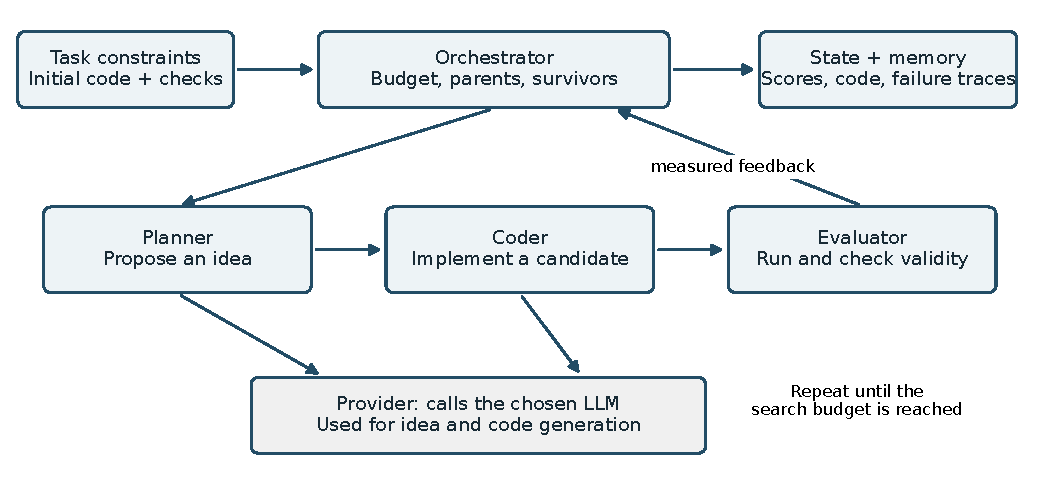
\includegraphics[width=\linewidth]{../../program_search/figures/framework.pdf}
\end{center}
\figcaption{fig:framework-zh}{依据官方架构和数据流资料绘制的解释性框架图。Provider 连接模型，Planner 提出修改，Coder 生成代码，Evaluator 执行检查，Orchestrator 管理选择、迁移与停止。\cite{architecture,dataflow} 保存配置和实际停止范围另见附录~\ref{app:online-zh}。}
\end{minipage}\par

\end{minipage}

一次迭代先固定任务接口、约束和评估器，再在允许修改的代码区域产生候选。评估器执行它，记录分数或失败；搜索机制据此选择后续父程序。Island GA 让多个群体分开搜索并偶尔交换候选，有助于保留不同方向，但频繁迁移也可能让它们趋同。记忆和反思能复用经验，却需要额外检索和可靠性控制。\cite{islands,memory}

本研究选择单位正方形内 26 个圆的布局任务。\cite{benchmark,circle} 对圆心 $\boldsymbol c_i=(x_i,y_i)$ 和半径 $r_i$，
\begin{align}
\max_{\{\boldsymbol c_i,r_i\}_{i=1}^{26}}\quad
&S=\sum_{i=1}^{26}r_i, \label{eq:circle-objective-zh}\\
\text{满足}\quad
&r_i\ge0,\quad r_i\le x_i\le1-r_i,\quad r_i\le y_i\le1-r_i,\\
&\|\boldsymbol c_i-\boldsymbol c_j\|_2\ge r_i+r_j,\quad i<j.
\end{align}
目标是\key{半径之和}，不是覆盖面积。评估还要求有限的 $(26,2)$ 圆心数组和 $(26,)$ 半径数组。只看图片是否紧密，不能替代几何检查。

在线实验使用真实 \code{deepseek-v4-flash} 调用、种子 42，保存预算为 2 个岛、每岛初始目标 2 个候选及 2 代演化，最多 2 个并发请求，Coder 输出上限为 32,768 tokens。2026 年 10 月 31 日修正版的记录覆盖初始化、第 1 代及第 2 代开始；最后导出后手动停止。本文统计实际完成的评估，不把保存预算写成已经全部执行的次数。



保存配置采用锦标赛父代选择、截断式保留，变异率为 0.3、交叉率为 0.5、精英比例为 0.2；迁移间隔为 1，拓扑为环形。Coder 温度为 0.7，保存的上下文上限为 8,192。评估器不重试。记忆提取被关闭，但运行日志仍出现评估轨迹嵌入，因此不能据此断言所有记忆操作均未发生。这些配置限定了实验解释范围，不能保证另一时点的托管服务产生相同程序。
